
%(BEGIN_QUESTION)
% Copyright 2006, Tony R. Kuphaldt, released under the Creative Commons Attribution License (v 1.0)
% This means you may do almost anything with this work of mine, so long as you give me proper credit

Explain the operation of this control circuit, including the functions of both potentiometers, and a determination of where those potentiometers should be set to achieve the ``tightest'' temperature control (resulting in the closest adherence to a setpoint temperature over time).  Recall that a {\it thermocouple} generates a small voltage proportional to temperature:

$$\includegraphics[width=15.5cm]{i01451x01.eps}$$

\underbar{file i01451}
%(END_QUESTION)





%(BEGIN_ANSWER)

Two potentiometers provide dual setpoints for the voltage comparators to act upon.  If the process variable signal (the thermocouple's output voltage) is less than the lower setpoint, the lower op-amp saturates ``high,'' activating the ``Set'' input of the S-R latch and engaging power to the heating element.

When the oven temperature is between the two setpoints (LSP $<$ PV $<$ USP), both op-amp outputs will be in the ``low'' state, and the S-R latch will hold its last output state on Q. 

When the process variable exceeds the upper setpoint, the upper op-amp saturates ``high,'' activating the ``Reset'' input of the S-R latch and disengaging power to the heating element.

\vskip 10pt

In summary, this is a simple {\it differential-gap} control system for a cookie oven.  For tightest temperature control, set the LSP potentiometer to maximum (full {\it up}) and the USP potentiometer to minimum (full {\it down}).

%(END_ANSWER)





%(BEGIN_NOTES)

$$\includegraphics[width=15.5cm]{i01451x02.eps}$$

\vskip 20pt \vbox{\hrule \hbox{\strut \vrule{} {\bf Virtual Troubleshooting} \vrule} \hrule}

This question is a good candidate for a ``Virtual Troubleshooting'' exercise.  Presenting the diagram to students, you first imagine in your own mind a particular fault in the system.  Then, you present one or more symptoms of that fault (something noticeable by an operator or other user of the system).  Students then propose various diagnostic tests to perform on this system to identify the nature and location of the fault, as though they were technicians trying to troubleshoot the problem.  Your job is to tell them what the result(s) would be for each of the proposed diagnostic tests, documenting those results where all the students can see.

During and after the exercise, it is good to ask students follow-up questions such as:

\begin{itemize}
\item{} What does the result of the last diagnostic test tell you about the fault?
\item{} Suppose the results of the last diagnostic test were different.  What then would that result tell you about the fault?
\item{} Is the last diagnostic test the best one we could do?
\item{} What would be the ideal order of tests, to diagnose the problem in as few steps as possible?
\end{itemize}

%INDEX% Control, basics: differential gap control (electronic)

%(END_NOTES)


